\subsection{Trusses}

\begin{figure}
  \begin{center}
  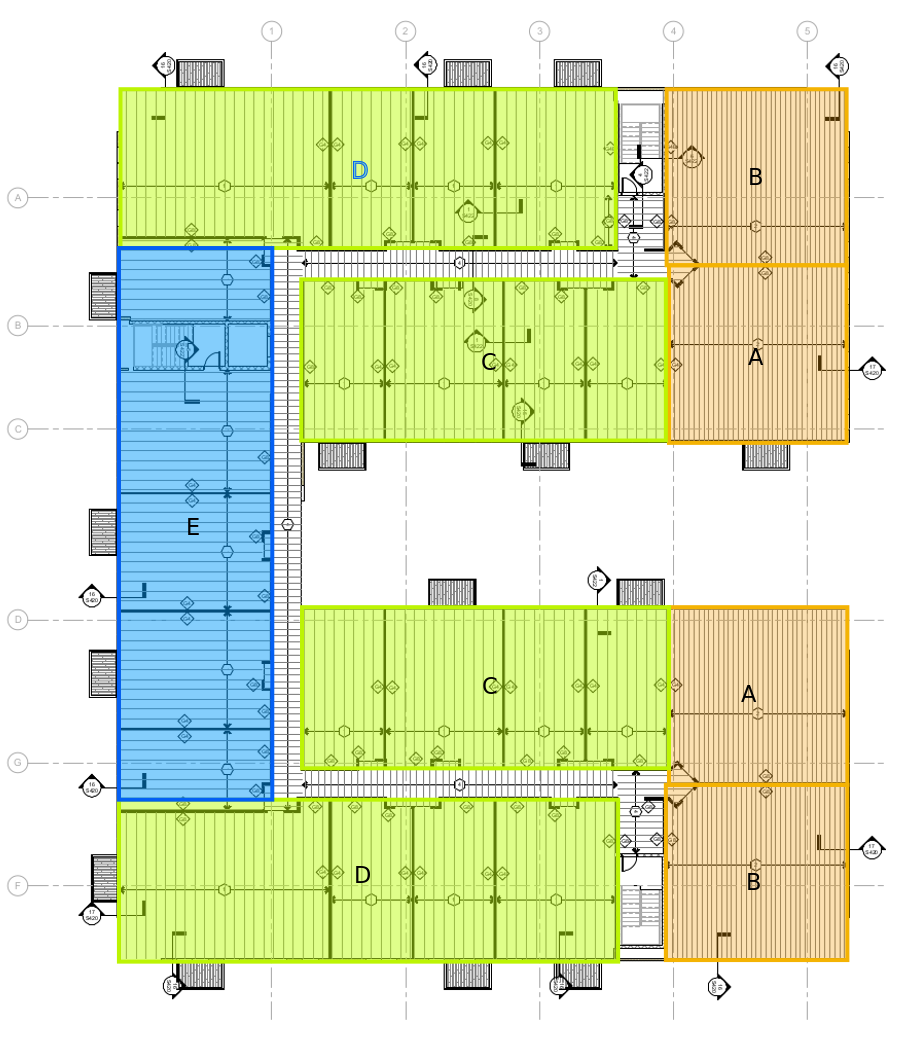
\includegraphics[width=120mm]{figures/3rd_floor_truss_key_plan}
  \end{center}
  \caption{Trusses key plan.}\label{fg_3rd_floor_truss_key_plan}
\end{figure}

\subsubsection{Trusses A and B. Roof}
The deflection results for those trusses (see figure \ref{fg_roof_truss_AB}) are as follows \footnote{The load combinations are listed in \ref{sc_load_combinations}.}:

\begin{center}
  \begin{scriptsize}
  \begin{tabular}{|l|c|c|c|c|c|c|}
    \hline
    \textbf{Load} & \textbf{truss} & \multicolumn{2}{c|}{\textbf{deflection}} & \textbf{truss} & \multicolumn{2}{c|}{\textbf{deflection}} \\
    \hline
EQ1608 & roof(A): & -1.94 mm & (L/5782; L= 11.22 m) & roof(B): &-1.12 mm & (L/9586; L= 10.77 m) \\
EQ1609 & roof(A): & -5.63 mm & (L/1994; L= 11.22 m) & roof(B): & -3.82 mm & (L/2819; L= 10.77 m) \\
EQ1610 & roof(A): & -9.66 mm & (L/1161; L= 11.22 m) & roof(B): & -6.76 mm & (L/1591; L= 10.77 m) \\
EQ1611 & roof(A): & -10.49 mm & (L/1069; L= 11.22 m) & roof(B): & -7.38 mm & (L/1459; L= 10.77 m) \\
EQ1612 & roof(A): & 0.99 mm & (L/11391; L= 11.22 m) & roof(B): & 1.02 mm & (L/10598; L= 10.77 m) \\
EQ1613 & roof(A): & -8.30 mm & (L/1352; L= 11.22 m) & roof(B): & -5.77 mm & (L/1865; L= 10.77 m) \\
EQ1615 & roof(A): & 1.76 mm & (L/6370; L= 11.22 m) & roof(B): & 1.47 mm & (L/7348; L= 10.77 m) \\
LIVE & roof(A): & -3.69 mm & (L/3044; L= 11.22 m) & roof(B): & -2.69 mm & (L/3995; L= 10.77 m) \\
\hline
  \end{tabular}
  \end{scriptsize}
\end{center}

\noindent The truss depth is allways greater than 24 inches due to the geometry of the roof. The spacing of the trusses is 24 inches.

\begin{align}
\Delta_{LL,A} &= 3.69\ mm= \frac{L}{3044} < \frac{L}{540} \implies OK \\
\Delta_{LL,B} &= 2.69\ mm= \frac{L}{3995} < \frac{L}{540} \implies OK \\
\Delta_{TL,A} &= 10.49\ mm= \frac{L}{1069} < \frac{L}{360} \implies OK \\
\Delta_{TL,B} &= 7.38\ mm= \frac{L}{1459} < \frac{L}{360} \implies OK
\end{align}

\begin{figure}
  \begin{center}
  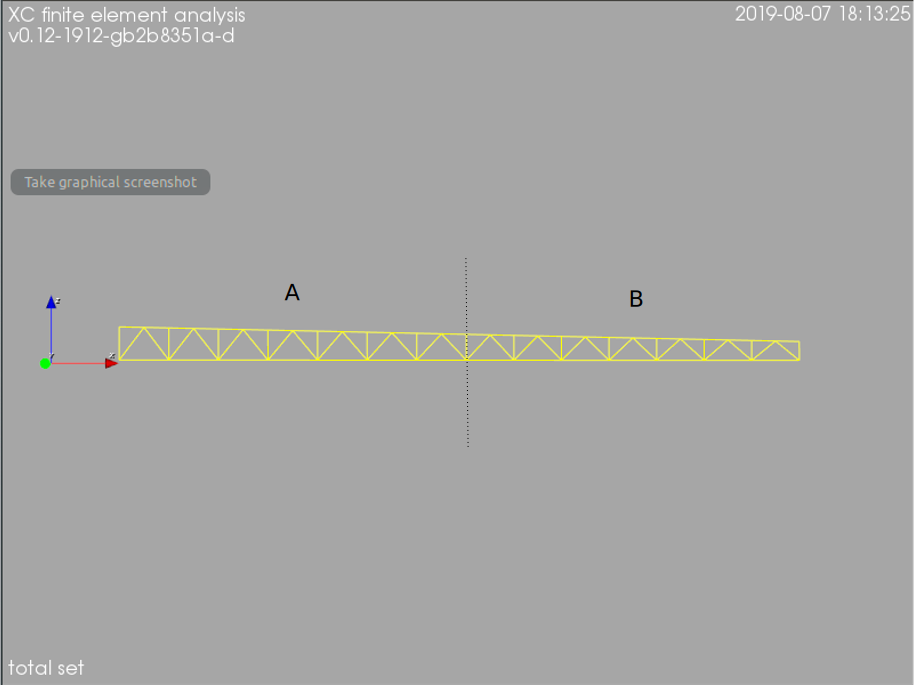
\includegraphics[width=120mm]{figures/roof_truss_AB}
  \end{center}
  \caption{Roof trusses at zones A and B (see key plan in figure \ref{fg_3rd_floor_truss_key_plan}).}\label{fg_roof_truss_AB}
\end{figure}

\subsubsection{Trusses A and B. Third floor}
The deflection results for those trusses (see figure \ref{fg_floor_truss_AB}) are as follows:

\begin{center}
  \begin{scriptsize}
  \begin{tabular}{|l|c|c|c|c|c|c|}
    \hline
    \textbf{Load} & \textbf{truss} & \multicolumn{2}{c|}{\textbf{deflection}} & \textbf{truss} & \multicolumn{2}{c|}{\textbf{deflection}} \\
    \hline
EQ1608 & A & -9.14 mm & (L/1228; L= 11.22 m)  & B & -7.75 mm & (L/1389; L= 10.77 m) \\
EQ1609 & A & -26.45 mm & (L/424; L= 11.22 m) & B & -22.46 mm & (L/479; L= 10.77 m) \\
EQ1610 & A & -9.13 mm & (L/1228; L= 11.22 m) & B & -7.74 mm & (L/1389; L= 10.77 m) \\
EQ1611 & A & -22.12 mm & (L/507; L= 11.22 m) & B & -18.78 mm & (L/573; L= 10.77 m) \\
EQ1612 & A & -9.14 mm & (L/1228; L= 11.22 m) & B & -7.75 mm & (L/1389; L= 10.77 m) \\
EQ1613 & A & -22.12 mm & (L/507; L= 11.22 m) & B & -18.78 mm & (L/573; L= 10.77 m) \\
EQ1615 & A & -5.48 mm & (L/2047; L= 11.22 m) & B & -4.65 mm & (L/2315; L= 10.77 m) \\
LIVE & A & -17.32 mm & (L/648; L= 11.22 m) & B & -14.71 mm & (L/731; L= 10.77 m) \\
\hline
  \end{tabular}
  \end{scriptsize}
\end{center}

\noindent The truss depth is 24 inches and the spacing of the trusses is 12 inches.

\begin{align}
\Delta_{LL,A} &= 17.32\ mm= \frac{L}{648} < \frac{L}{540} \implies OK \\
\Delta_{LL,B} &= 14.71\ mm= \frac{L}{731} < \frac{L}{540} \implies OK \\
\Delta_{TL,A} &= 26.45\ mm= \frac{L}{424} < \frac{L}{360} \implies OK \\
\Delta_{TL,B} &= 22.46\ mm= \frac{L}{479} < \frac{L}{360} \implies OK
\end{align}


\begin{figure}
  \begin{center}
  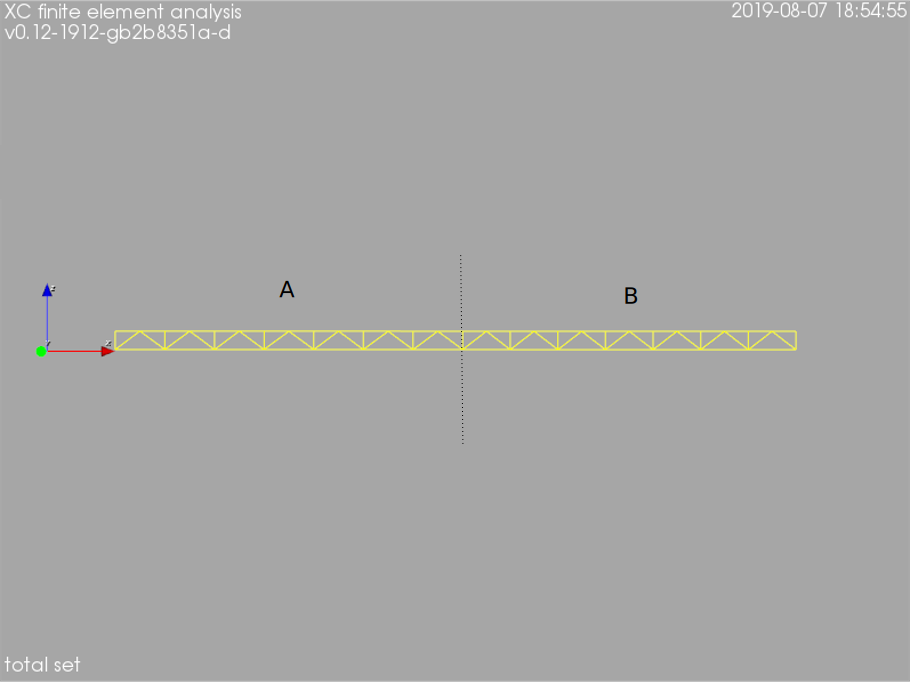
\includegraphics[width=120mm]{figures/floor_truss_AB}
  \end{center}
  \caption{Third floor trusses at zones A and B (see key plan in figure \ref{fg_3rd_floor_truss_key_plan}).}\label{fg_floor_truss_AB}
\end{figure}

\subsubsection{Trusses A and B. Second floor}
The deflection results for those trusses (see figure \ref{fg_2nd_floor_truss_AB}) are as follows:

\begin{center}
  \begin{scriptsize}
  \begin{tabular}{|l|c|c|c|c|c|c|}
    \hline
    \textbf{Load} & \textbf{truss} & \multicolumn{2}{c|}{\textbf{deflection}} & \textbf{truss} & \multicolumn{2}{c|}{\textbf{deflection}} \\
    \hline
EQ1608& A &-8.13  mm & (L/1282; L= 10.42 m) & B &  -6.81  mm & (L/1464; L= 9.97 m)\\
EQ1609& A &-23.51  mm & (L/443; L= 10.42 m) & B &  -19.71  mm & (L/505; L= 9.97 m)\\
EQ1610& A &-8.13  mm & (L/1282; L= 10.42 m) & B &  -6.81  mm & (L/1464; L= 9.97 m)\\
EQ1611& A &-19.66  mm & (L/530; L= 10.42 m) & B &  -16.48  mm & (L/604; L= 9.97 m)\\
EQ1612& A &-8.13  mm & (L/1282; L= 10.42 m) & B &  -6.81  mm & (L/1464; L= 9.97 m)\\
EQ1613& A &-19.66  mm & (L/530; L= 10.42 m) & B &  -16.48  mm & (L/604; L= 9.97 m)\\
EQ1615& A &-4.88  mm & (L/2136; L= 10.42 m) & B &  -4.08  mm & (L/2440; L= 9.97 m)\\
LIVE& A &-15.38  mm & (L/677; L= 10.42 m) & B & -12.90  mm & (L/772; L= 9.97 m)\\
\hline
  \end{tabular}
  \end{scriptsize}
\end{center}

\noindent The truss depth is 22 inches and the spacing of the trusses is 12 inches.

\begin{align}
\Delta_{LL,A} &= 15.38\ mm= \frac{L}{677} < \frac{L}{540} \implies OK \\
\Delta_{LL,B} &= 12.90\ mm= \frac{L}{772} < \frac{L}{540} \implies OK \\
\Delta_{TL,A} &= 23.51\ mm= \frac{L}{443} < \frac{L}{360} \implies OK \\
\Delta_{TL,B} &= 19.71\ mm= \frac{L}{505} < \frac{L}{360} \implies OK
\end{align}

\begin{figure}
  \begin{center}
  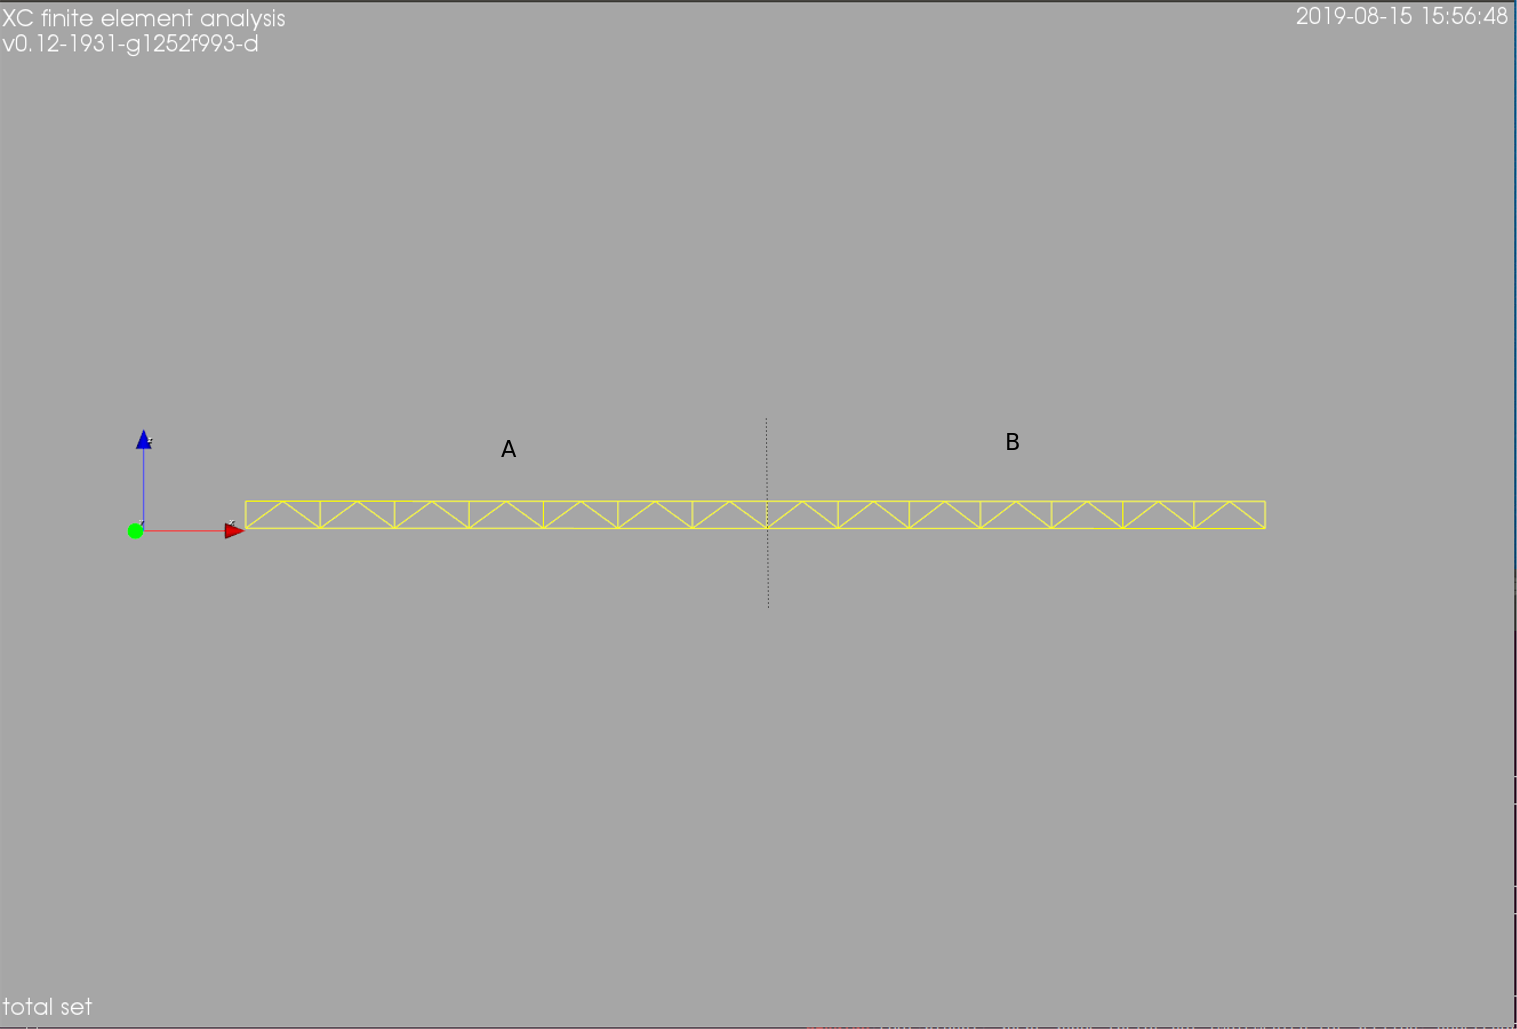
\includegraphics[width=120mm]{figures/2nd_floor_truss_AB}
  \end{center}
  \caption{Second floor trusses at zones A and B (see key plan in figure \ref{fg_3rd_floor_truss_key_plan}).}\label{fg_2nd_floor_truss_AB}
\end{figure}

\subsubsection{Trusses C and D. Roof}
The deflection results for those trusses (see figure \ref{fg_roof_truss_CD}) are as follows:

\begin{center}
  \begin{scriptsize}
  \begin{tabular}{|l|c|c|c|c|c|c|}
    \hline
    \textbf{Load} & \textbf{truss} & \multicolumn{2}{c|}{\textbf{deflection}} & \textbf{truss} & \multicolumn{2}{c|}{\textbf{deflection}} \\
    \hline
EQ1608 & roof(C) & -2.92 mm & (L/3420; L= 10.00 m) & roof(D) & -5.24 mm & (L/1822; L= 9.55 m) \\
EQ1609 & roof(C) & -7.42 mm & (L/1347; L= 10.00 m) & roof(D) & -11.87 mm & (L/803; L= 9.55 m) \\
EQ1610 & roof(C) & -12.34 mm & (L/810; L= 10.00 m) & roof(D) & -19.13 mm & (L/498; L= 9.55 m) \\
EQ1611 & roof(C) & -13.36 mm & (L/748; L= 10.00 m) & roof(D) & -20.64 mm & (L/462; L= 9.55 m) \\
EQ1612 & roof(C) & 0.64 mm & (L/15512; L= 10.00 m) & roof(D) & 0.03 mm & (L/323264; L= 9.55 m) \\
EQ1613 & roof(C) & -10.68 mm & (L/936; L= 10.00 m) & roof(D) & -16.69 mm & (L/572; L= 9.55 m) \\
EQ1615 & roof(C) & 1.81 mm & (L/5512; L= 10.00 m) & roof(D) & 2.12 mm & (L/4493; L= 9.55 m) \\
LIVE & roof(C) & -4.50 mm & (L/2224; L= 10.00 m) & roof(D) & -6.64 mm & (L/1438; L= 9.55 m) \\
\hline
  \end{tabular}
  \end{scriptsize}
\end{center}

\noindent The truss depth is allways greater than 24 inches due to the geometry of the roof. The spacing of the trusses is 24 inches. The spacing of the joists is 32 inches. 

\begin{align}
\Delta_{LL,C} &= 4.50\ mm= \frac{L}{2224} < \frac{L}{540} \implies OK \\
\Delta_{LL,D} &= 6.64\ mm= \frac{L}{772} < \frac{L}{540} \implies OK \\
\Delta_{TL,C} &= 13.36\ mm= \frac{L}{748} < \frac{L}{360} \implies OK \\
\Delta_{TL,D} &= 20.64\ mm= \frac{L}{462} < \frac{L}{360} \implies OK
\end{align}

\begin{figure}
  \begin{center}
  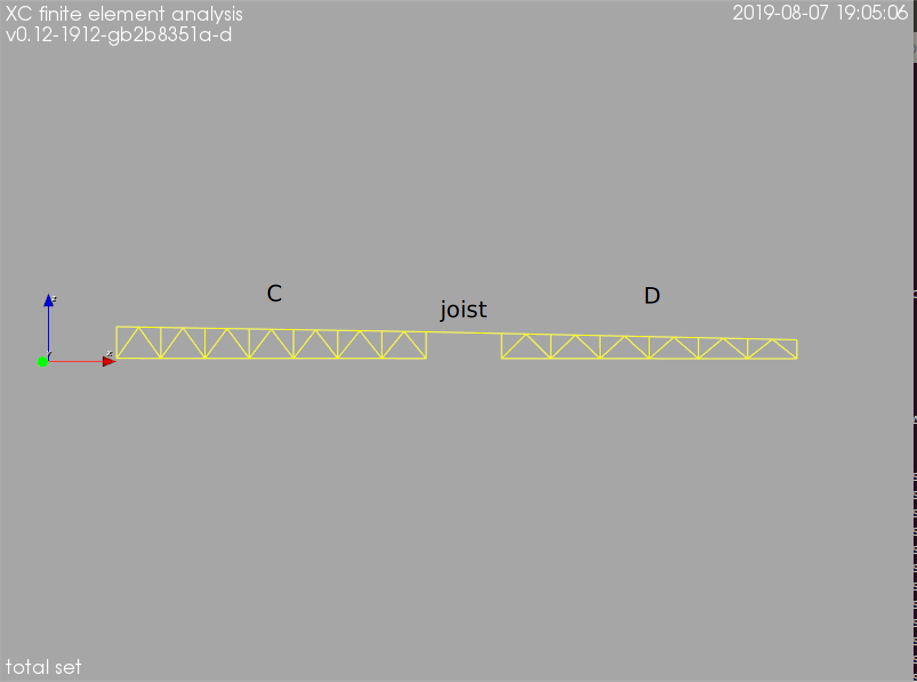
\includegraphics[width=120mm]{figures/roof_truss_CD}
  \end{center}
  \caption{Roof trusses at zones C and D (see key plan in figure \ref{fg_3rd_floor_truss_key_plan}).}\label{fg_roof_truss_CD}
\end{figure}

\subsubsection{Trusses C and D. Third floor}
The deflection results for those trusses (see figure \ref{fg_floor_truss_CD}) are as follows:

\begin{center}
  \begin{scriptsize}
  \begin{tabular}{|l|c|c|c|c|c|c|}
    \hline
    \textbf{Load} & \textbf{truss} & \multicolumn{2}{c|}{\textbf{deflection}} & \textbf{truss} & \multicolumn{2}{c|}{\textbf{deflection}} \\
    \hline
EQ1608 & C & -10.00 mm & (L/982; L= 9.82 m) & D & -8.93 mm & (L/1048; L= 9.37 m) \\
EQ1609 & C & -26.93 mm & (L/364; L= 9.82 m) & D & -24.04 mm & (L/389; L= 9.37 m) \\
EQ1610 & C & -10.00 mm & (L/982; L= 9.82 m) & D & -8.93 mm & (L/1048; L= 9.37 m) \\
EQ1611 & C & -22.70 mm & (L/432; L= 9.82 m) & D & -20.26 mm & (L/462; L= 9.37 m) \\
EQ1612 & C & -10.00 mm & (L/982; L= 9.82 m) & D & -8.93 mm & (L/1048; L= 9.37 m) \\
EQ1613 & C & -22.70 mm & (L/432; L= 9.82 m) & D & -20.26 mm & (L/462; L= 9.37 m) \\
EQ1615 & C & -6.00 mm & (L/1636; L= 9.82 m) & D & -5.36 mm & (L/1747; L= 9.37 m) \\
LIVE & C & -16.93 mm & (L/580; L= 9.82 m) & D & -15.11 mm & (L/620; L= 9.37 m) \\
\hline
  \end{tabular}
  \end{scriptsize}
\end{center}

\noindent The truss depths are 24 inches for the C truss 22 inches for the D truss. The spacing of the trusses is 24 inches. The spacing of the joists is 32 inches. 

\begin{align}
\Delta_{LL,C} &= 16.93\ mm= \frac{L}{580} < \frac{L}{540} \implies OK \\
\Delta_{LL,D} &= 15.11\ mm= \frac{L}{620} < \frac{L}{540} \implies OK \\
\Delta_{TL,C} &= 26.93\ mm= \frac{L}{364} < \frac{L}{360} \implies OK \\
\Delta_{TL,D} &= 24.04\ mm= \frac{L}{389} < \frac{L}{360} \implies OK
\end{align}

\begin{figure}
  \begin{center}
  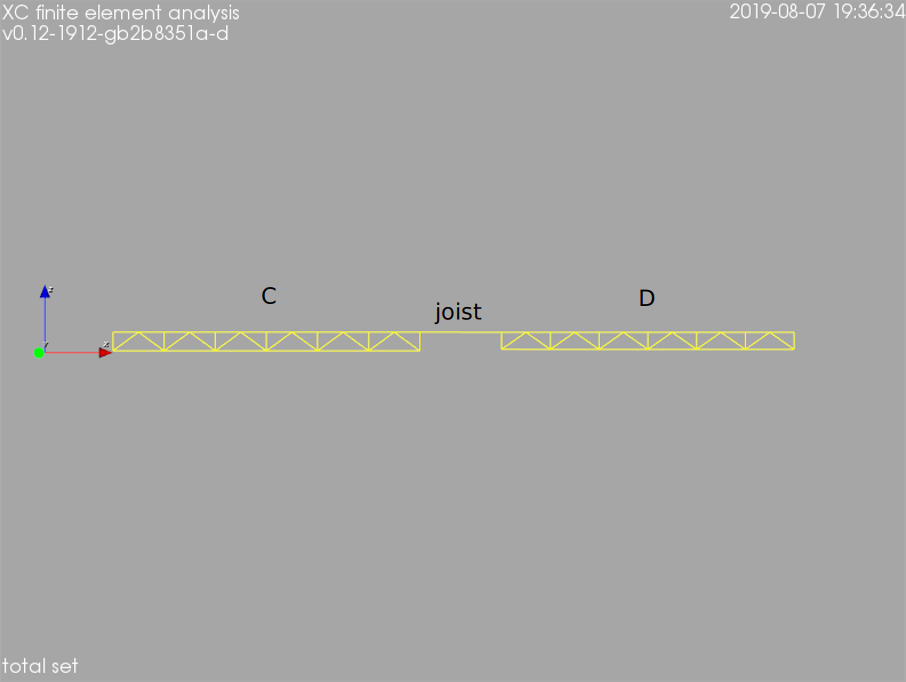
\includegraphics[width=120mm]{figures/floor_truss_CD}
  \end{center}
  \caption{Third floor trusses at zones C and D (see key plan in figure \ref{fg_3rd_floor_truss_key_plan}).}\label{fg_floor_truss_CD}
\end{figure}

\subsubsection{Trusses C and D. Second floor}
The deflection results for those trusses (see figure \ref{fg_2nd_floor_truss_CD}) are as follows:

\begin{center}
  \begin{scriptsize}
  \begin{tabular}{|l|c|c|c|c|c|c|}
    \hline
    \textbf{Load} & \textbf{truss} & \multicolumn{2}{c|}{\textbf{deflection}} & \textbf{truss} & \multicolumn{2}{c|}{\textbf{deflection}} \\
    \hline
EQ1608& C &-8.43  mm & (L/1070; L= 9.02 m) & D & -9.01  mm & (L/1039; L= 9.37 m)\\
EQ1609& C &-22.70  mm & (L/397; L= 9.02 m) & D & -24.24  mm & (L/386; L= 9.37 m)\\
EQ1610& C &-8.43  mm & (L/1070; L= 9.02 m) & D & -9.01  mm & (L/1039; L= 9.37 m)\\
EQ1611& C &-19.14  mm & (L/471; L= 9.02 m) & D & -20.43  mm & (L/458; L= 9.37 m)\\
EQ1612& C &-8.43  mm & (L/1070; L= 9.02 m) & D & -9.01  mm & (L/1039; L= 9.37 m)\\
EQ1613& C &-19.14  mm & (L/471; L= 9.02 m) & D & -20.43  mm & (L/458; L= 9.37 m)\\
EQ1615& C &-5.06  mm & (L/1783; L= 9.02 m) & D & -5.41  mm & (L/1732; L= 9.37 m)\\
LIVE& C &-14.27  mm & (L/632; L= 9.02 m) & D & -15.23  mm & (L/614; L= 9.37 m)\\
\hline
  \end{tabular}
  \end{scriptsize}
\end{center}

\noindent The truss depths are 22 inches. The spacing of the trusses is 24 inches. The spacing of the joists is 32 inches. 

\begin{align}
\Delta_{LL,C} &= 14.27\ mm= \frac{L}{632} < \frac{L}{540} \implies OK \\
\Delta_{LL,D} &= 15.23\ mm= \frac{L}{614} < \frac{L}{540} \implies OK \\
\Delta_{TL,C} &= 22.70\ mm= \frac{L}{397} < \frac{L}{360} \implies OK \\
\Delta_{TL,D} &= 24.24\ mm= \frac{L}{386} < \frac{L}{360} \implies OK
\end{align}

\begin{figure}
  \begin{center}
  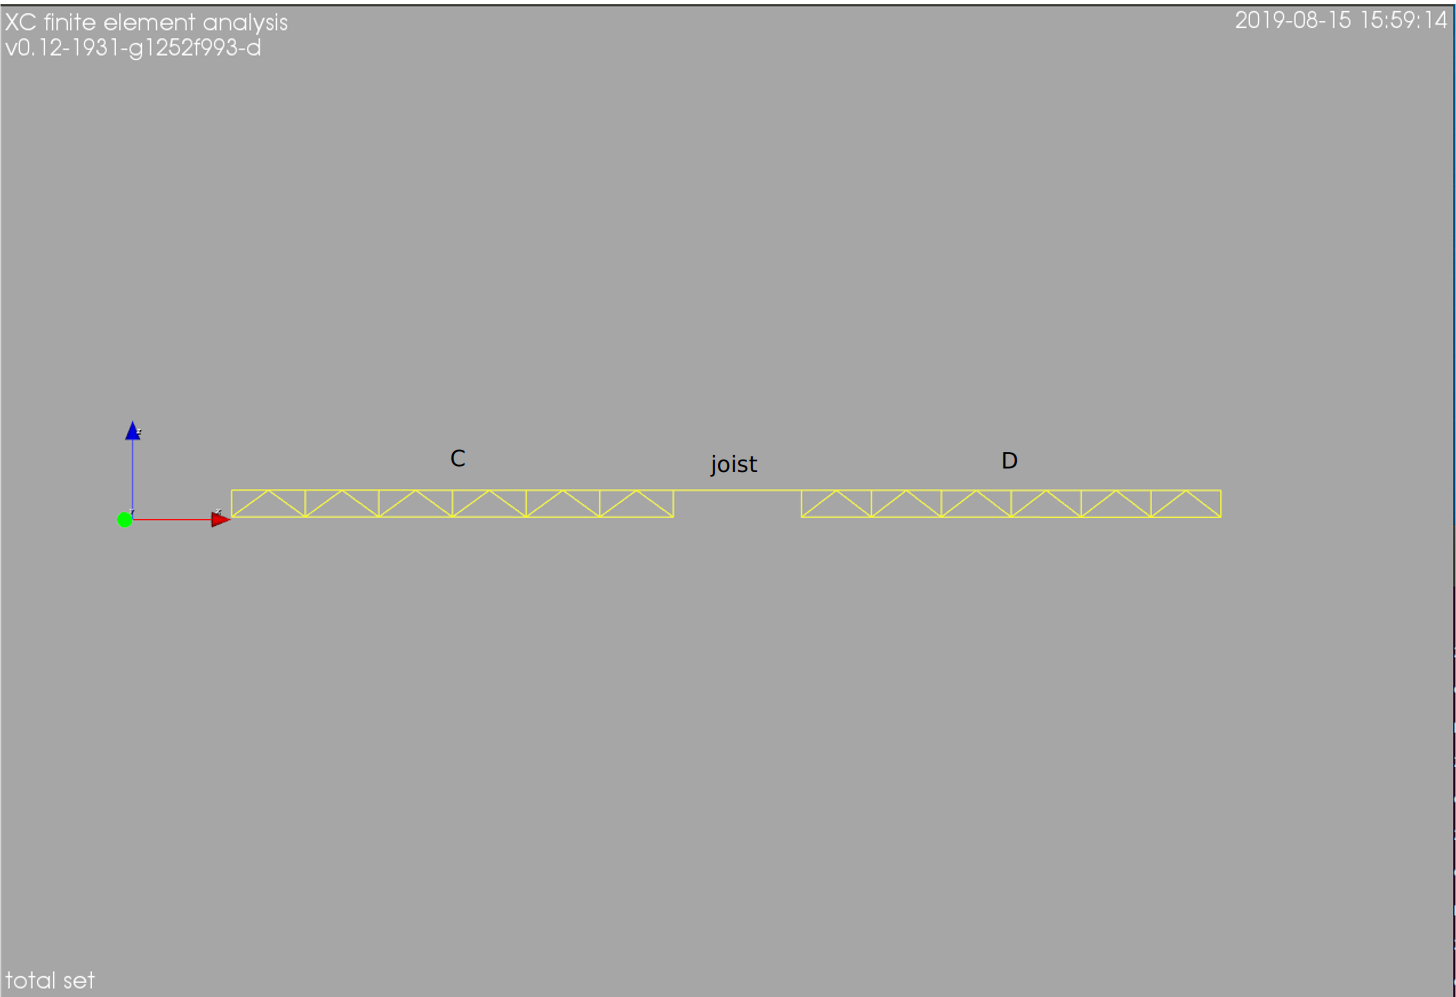
\includegraphics[width=120mm]{figures/2nd_floor_truss_CD}
  \end{center}
  \caption{Second floor trusses at zones C and D (see key plan in figure \ref{fg_3rd_floor_truss_key_plan}).}\label{fg_2nd_floor_truss_CD}
\end{figure}

\subsubsection{Truss E. Roof}
The deflection results for those trusses (see figure \ref{fg_roof_truss_E}) are as follows:

\begin{center}
  \begin{scriptsize}
  \begin{tabular}{|l|c|c|c|c|c|c|}
    \hline
    \textbf{Load} & \textbf{truss} & \multicolumn{2}{c|}{\textbf{deflection}} \\
    \hline
EQ1608 & 3E & -4.67 mm & (L/2025; L= 9.47 m) \\
EQ1609 & 3E & -11.56 mm & (L/819; L= 9.47 m) \\
EQ1610 & 3E & -19.09 mm & (L/496; L= 9.47 m) \\
EQ1611 & 3E & -20.65 mm & (L/458; L= 9.47 m) \\
EQ1612 & 3E & 0.79 mm & (L/11978; L= 9.47 m) \\
EQ1613 & 3E & -16.55 mm & (L/572; L= 9.47 m) \\
EQ1615 & 3E & 2.66 mm & (L/3559; L= 9.47 m) \\
LIVE & 3E & -6.89 mm & (L/1375; L= 9.47 m) \\
\hline
  \end{tabular}
  \end{scriptsize}
\end{center}

\noindent The truss depth is allways greater than 24 inches due to the geometry of the roof. The spacing of the trusses is 24 inches. The spacing of the joists is 32 inches.

\begin{align}
\Delta_{LL,E} &= 6.89\ mm= \frac{L}{1375} < \frac{L}{540} \implies OK \\
\Delta_{TL,E} &= 20.65\ mm= \frac{L}{458} < \frac{L}{360} \implies OK \\
\end{align}

\begin{figure}
  \begin{center}
  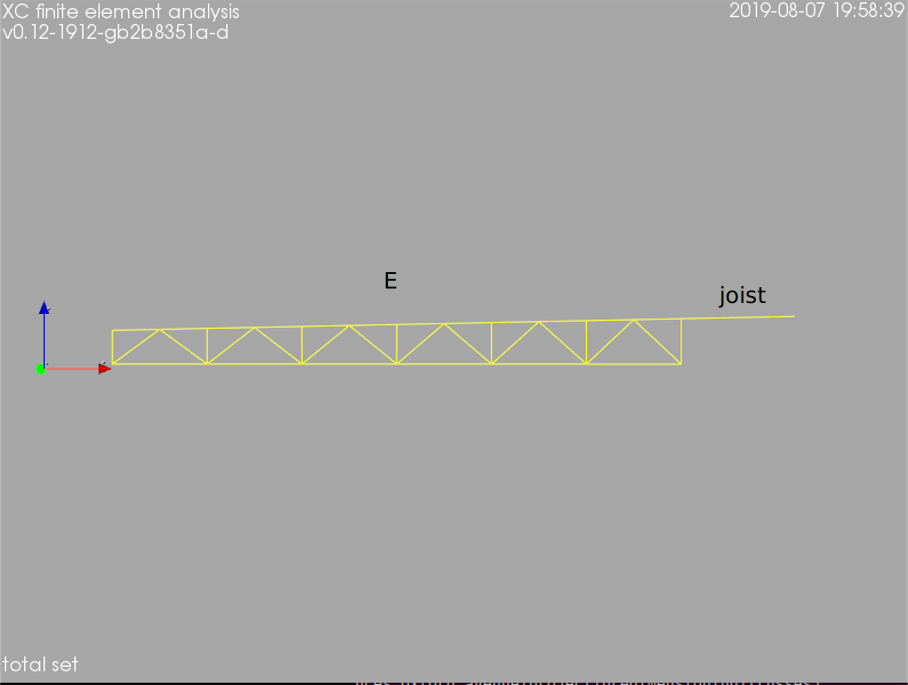
\includegraphics[width=120mm]{figures/roof_truss_E}
  \end{center}
  \caption{Roof truss at zone E (see key plan in figure \ref{fg_3rd_floor_truss_key_plan}).}\label{fg_roof_truss_E}
\end{figure}

\subsubsection{Truss E. Third floor}
The deflection results for those trusses (see figure \ref{fg_floor_truss_E}) are as follows:

\begin{center}
  \begin{scriptsize}
  \begin{tabular}{|l|c|c|c|c|c|c|}
    \hline
    \textbf{Load} & \textbf{truss} & \multicolumn{2}{c|}{\textbf{deflection}} \\
    \hline
EQ1608 & 2E & -8.65 mm & (L/1095; L= 9.47 m) \\
EQ1609 & 2E & -23.30 mm & (L/406; L= 9.47 m) \\
EQ1610 & 2E & -8.65 mm & (L/1095; L= 9.47 m) \\
EQ1611 & 2E & -19.63 mm & (L/482; L= 9.47 m) \\
EQ1612 & 2E & -8.65 mm & (L/1095; L= 9.47 m) \\
EQ1613 & 2E & -19.63 mm & (L/482; L= 9.47 m) \\
EQ1615 & 2E & -5.19 mm & (L/1825; L= 9.47 m) \\
LIVE & 2E & -14.65 mm & (L/646; L= 9.47 m) \\
\hline
  \end{tabular}
  \end{scriptsize}
\end{center}

\noindent The truss depth 24 inches. The spacing of the trusses is 24 inches and the spacing of the joists is 32 inches.

\begin{align}
\Delta_{LL,E} &= 14.65\ mm= \frac{L}{646} < \frac{L}{540} \implies OK \\
\Delta_{TL,E} &= 23.30\ mm= \frac{L}{406} < \frac{L}{360} \implies OK \\
\end{align}

\begin{figure}
  \begin{center}
  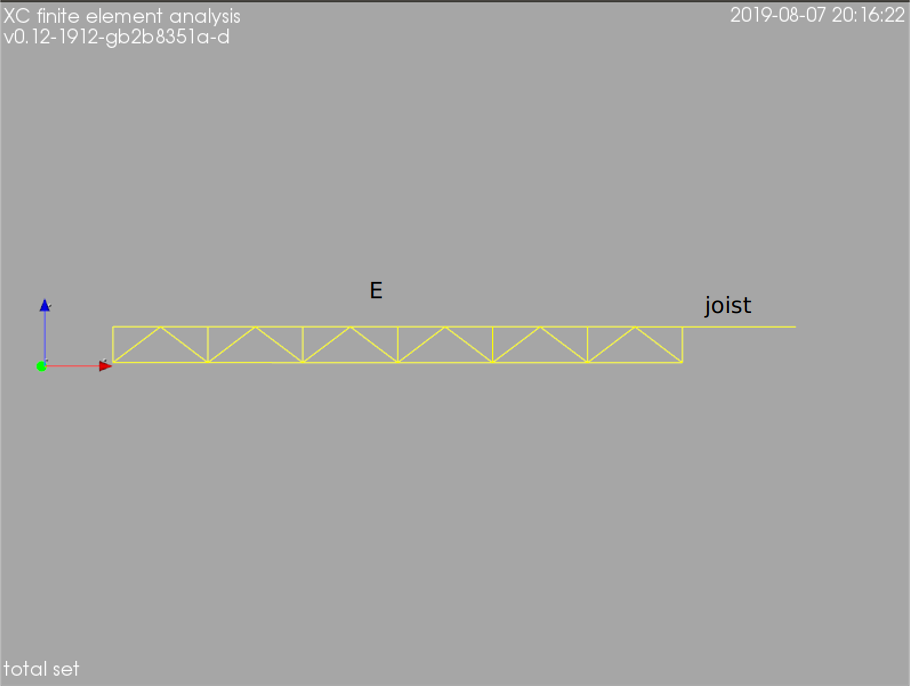
\includegraphics[width=120mm]{figures/floor_truss_E}
  \end{center}
  \caption{Third floor truss at zone E (see key plan in figure \ref{fg_3rd_floor_truss_key_plan}).}\label{fg_floor_truss_E}
\end{figure}

\subsubsection{Truss E. Second floor}
The deflection results for those trusses (see figure \ref{fg_2nd_floor_truss_E}) are as follows:

\begin{center}
  \begin{scriptsize}
  \begin{tabular}{|l|c|c|c|c|c|c|}
    \hline
    \textbf{Load} & \textbf{truss} & \multicolumn{2}{c|}{\textbf{deflection}} \\
    \hline
EQ1608 2E: -7.18  mm & (L/1208; L= 8.67 m)\\
EQ1609 2E: -19.34  mm & (L/448; L= 8.67 m)\\
EQ1610 2E: -7.18  mm & (L/1208; L= 8.67 m)\\
EQ1611 2E: -16.30  mm & (L/532; L= 8.67 m)\\
EQ1612 2E: -7.18  mm & (L/1208; L= 8.67 m)\\
EQ1613 2E: -16.30  mm & (L/532; L= 8.67 m)\\
EQ1615 2E: -4.31  mm & (L/2013; L= 8.67 m)\\
LIVE 2E: -12.16  mm & (L/713; L= 8.67 m)\\
\hline
  \end{tabular}
  \end{scriptsize}
\end{center}

\noindent The truss depth 22 inches. The spacing of the trusses is 24 inches and the spacing of the joists is 32 inches.

\begin{align}
\Delta_{LL,E} &= 12.16\ mm= \frac{L}{713} < \frac{L}{540} \implies OK \\
\Delta_{TL,E} &= 19.34\ mm= \frac{L}{448} < \frac{L}{360} \implies OK \\
\end{align}


\begin{figure}
  \begin{center}
  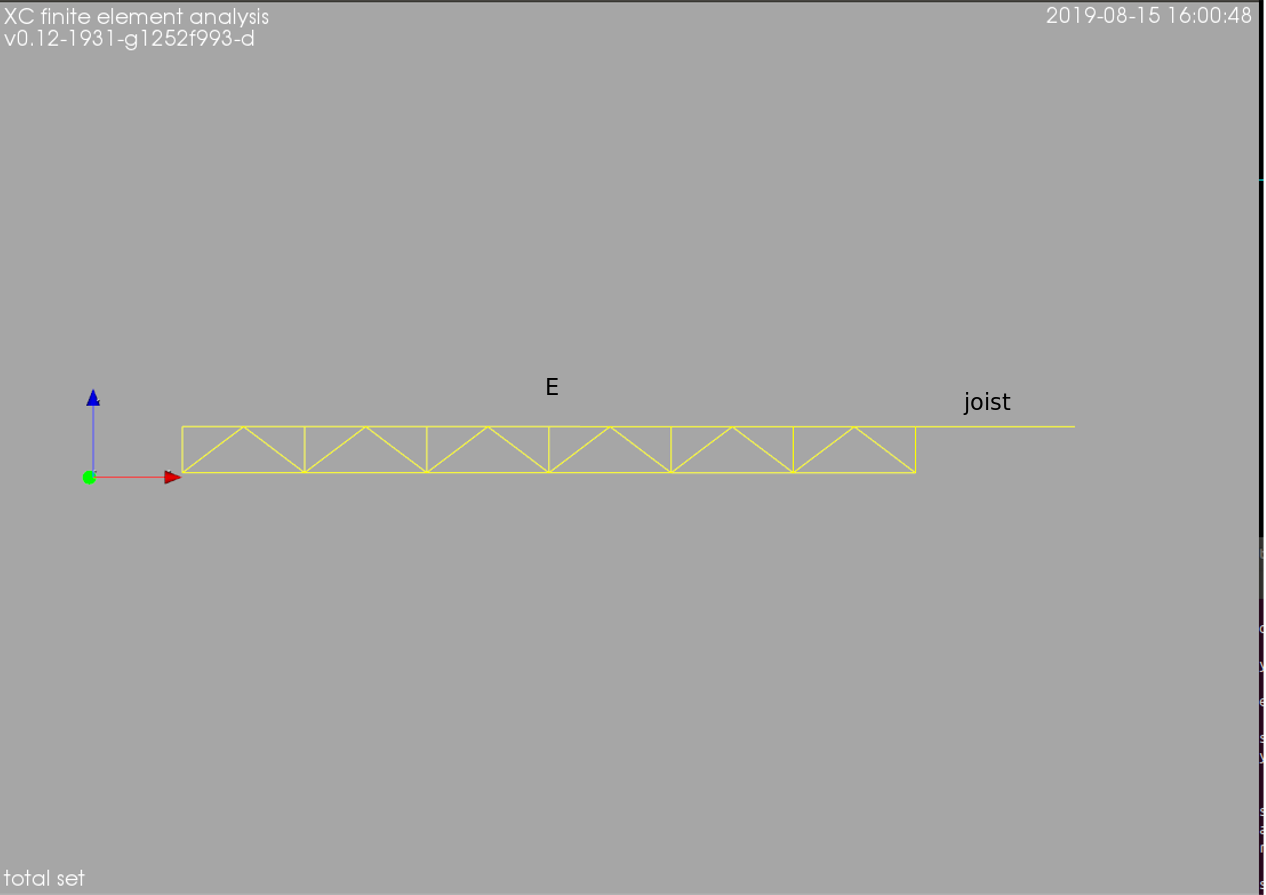
\includegraphics[width=120mm]{figures/2nd_floor_truss_E}
  \end{center}
  \caption{Second floor truss at zone E (see key plan in figure \ref{fg_3rd_floor_truss_key_plan}).}\label{fg_2nd_floor_truss_E}
\end{figure}
